\lab{Getting Started}{Getting Started}

The individual mandatory assignments (called ``labs'' in the following) in the second part of DM561 and DM562 aim to introduce to applications of Linear Algebra and to train your Python programming skills. There will be weekly programming tasks for which you have to submit a solution.

\section*{Submitting Assignments} % ===========================================

\subsection*{Labs}

Every lab has a corresponding specifications file with some code to get you started and to make your submission compatible with automated test drivers. The template code will be provided via IMADA Git Server at \url{https://git.imada.sdu.dk}. How to proceed in detail will be described below.


To submit a lab, modify the provided specifications file and use \texttt{git} to submit your solution (discussed in the next section).
The submissions will be automatically graded. 
For example, the first assignment (which will not be graded, and is just used to introduce you to the procedure of how you should submit your solutions and how your solution is graded) has the specifications file \texttt{asg0-onlytesting/onlytesting.py}.
To complete that assignment, provide your implementation in the file \texttt{asg0-onlytesting/asg0.py} and submit it via \texttt{git}.
After grading, you will be able to get access to a file called \texttt{asg0-onlytesting/grade.txt} with your score and some feedback. Each assignment will have a formal deadline. However we will provide testing results once every hour (at minute 00), such that you can improve your code. The grading will be based on your implementation at the exact time of the deadline of the assignment.


\begin{warn}
Do \textbf{not} move or rename the lab folders or the enclosed
specifications files; if you do, the test drivers will not be able to
find your assignment. Do \textbf{not} edit the file
\texttt{grade.txt}. This file is overwritten when you pull with git from
the remote server and must stay unchanged. 
\end{warn}


\newpage
\section*{Setup} % ============================================================

\begin{warn}
We strongly recommend using a Unix-based operating system (Mac or Linux) for the labs.
Unix has a true bash terminal, works well with git and python, and is the preferred platform for computational and data scientists.
It is possible to do this curriculum with Windows, but expect some road bumps along the way. We will ensure that all the exercises can be solved in the IMADA Computer Lab. You can use your own environment, but you should not expect that we are able to answer your environment specific questions.
\end{warn}

Code has to be submitted using git. 

\subsection*{Setup With Git} % ------------------------------------------------

\emph{Git} is a program that manages updates between an online code
repository and the copies of the repository, called \emph{clones},
stored locally on computers. Git is installed in the IMADA Computer
Lab. The instructions given below in this document should be enough for
the needs in this course. The tutorials linked below will provide much
more information than needed in this course. Nevertheless, git is an industry-standard collaboration tool, and being able to use it efficiently is an asset.

If you decide to use your own computer, and git is not already installed on your computer, you can download it at \url{http://git-scm.com/downloads} (or use the installation procedure of your specific system).
If you have never used git, you might want to read a few of the following resources.
\begin{itemize}
\item Official git tutorial: \url{https://git-scm.com/docs/gittutorial}
\item Bitbucket git tutorials: \url{https://www.atlassian.com/git/tutorials}
\item GitHub git cheat sheet: \href{https://services.github.com/on-demand/downloads/github-git-cheat-sheet.pdf}{\texttt{services.github.com/.../github-git-cheat-sheet.pdf}}
\item GitLab git tutorial: \url{https://docs.gitlab.com/ce/gitlab-basics/start-using-git.html}
\item Codecademy git lesson: \url{https://www.codecademy.com/learn/learn-git}
\item Training video series by GitHub: \href{https://www.youtube.com/playlist?list=PLg7s6cbtAD15G8lNyoaYDuKZSKyJrgwB-}{\texttt{https://www.youtube.com/playlist?list=PLg7.../}}
\end{itemize}

There are many websites for hosting online git repositories. IMADA has its own server for hosting git repositories  \url{https://git.imada.sdu.dk}. While not needed for submitting your code, you can login to the webpage using your university account name and the same password as you use for reading your mail or logging into blackboard. Choose as authentication source ``SDU''. See Fig.~\ref{fig:gogs} for an example. Via the webpage you will always be able to see the state of your code that will be used for auto-grading.

\begin{figure}
  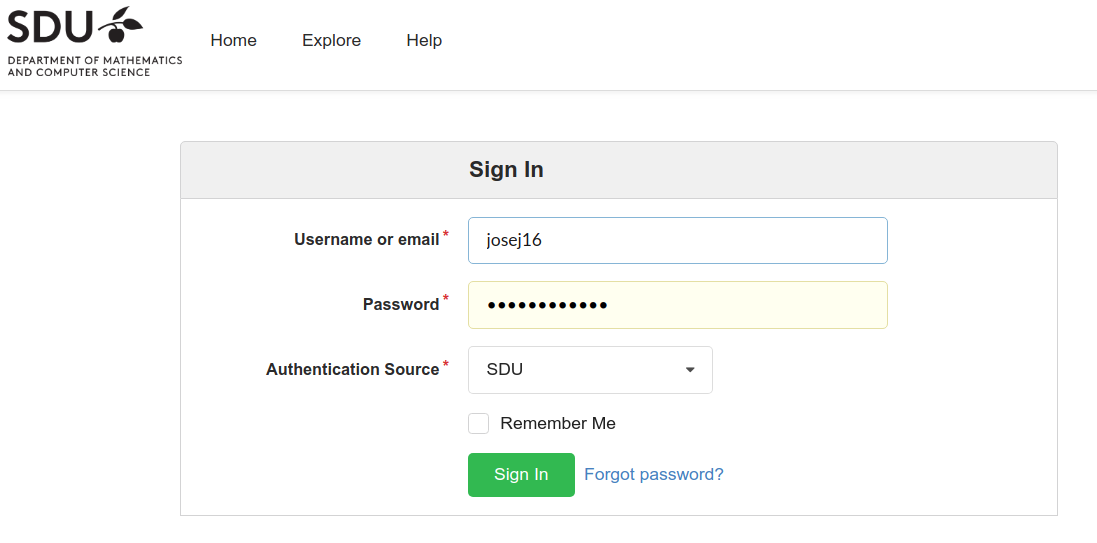
\includegraphics[width=\textwidth]{gogs}
  \caption{IMADA Git Server (Gogs) login page}
  \label{fig:gogs}
\end{figure}

\begin{enumerate}

\item \emph{Clone your existing repository}.

  Usually, you have to create a repository. However, we already created a repository for each student of DM561 and DM562. You will not have to create any repositories, but only clone it.
  
\item \emph{Connect your folder to the new repository}.
\label{step:connect-folder}\label{step:download-data}
In a shell application (Terminal on Linux or Mac, or Git Bash (\url{https://gitforwindows.org/}) on Windows), enter the following commands (we will use the student with the username ``josej16'' as example, of course you have to change this.

\begin{lstlisting}
# Navigate to the folder where you want to store your files
$ <b<cd>b> /path/to/folder  # cd means 'change directory'.

# Make sure you are in the right place.
$ <b<pwd>b>                 # pwd means 'print working directory'.
/path/to/folder

# Record your credentials (has to be done once only).
$ git config --local user.name "Jonathan S. Ejejej"
$ git config --local user.email "josej16@student.sdu.dk"

# Clone the repository we provided

$ git clone https://git.imada.sdu.dk/DM561-DM562-2019/josej16-repo.git

Cloning into 'josej16-repo'...
Username for 'https://git.imada.sdu.dk': josej16
Password for 'https://josej16@git.imada.sdu.dk': ********
remote: Counting objects: 48, done.
remote: Compressing objects: 100% (44/44), done.
remote: Total 48 (delta 16), reused 0 (delta 0)
Unpacking objects: 100% (48/48), done.
$ ls 
josej16-repo

$ cd josej16-repo
$ ls -rtl
-rw------- 1 josej16 josej16   66 Oct 31 19:48 README.md
-rw------- 1 josej16 josej16  134 Oct 31 19:48 Info.md
drwx------ 2 josej16 josej16 4096 Oct 31 19:48 asg0-onlytesting
\end{lstlisting}


\item \emph{Install Python package dependencies}.
\label{step:install-dependencies}
Some of the labs require third-party Python packages that you might not have installed on your system. If they are missing you will see an error message similar to 
\begin{lstlisting}
$ python test.py 
Traceback (most recent call last):
  File "test.py", line 1, in <module>
    import matplotlib
ImportError: No module named matplotlib
\end{lstlisting}

You can easily install missing packages via

\begin{lstlisting}
$ pip3 install --user matplotlib
Collecting matplotlib
  Downloading https://files.pythonhosted.org/packages/b2/58/5842588fa67b45ffb451c4c98eda283c0c42b8f2c5e503e4f6d9ff3c3a63/matplotlib-3.0.1-cp35-cp35m-manylinux1_x86_64.whl (12.9MB)
  [...]
  \end{lstlisting}

\end{enumerate}

%\subsection*{Setup Without Git} % ---------------------------------------------

Note, that you must have git installed in order to i.) get the data files for each lab and ii.) to submit you solution. Git is installed in the Computer Lab --- if you want to install it within your own environment, \url{http://git-scm.com/downloads} is a good starting point.

\section*{Using Git} % ========================================================

Git manages the history of a file system through \emph{commits}, or checkpoints.
Use \li{git status} to see the files that have been changed since the last commit.
These changes are then moved to the (local) \emph{staging area} (a list of files for the next commit) with \li{git add <filename(s)>}.
Record the changes in the staging area with the command \li{git commit -m "<A brief message describing the changes>"}.

All of these commands are done within a ``clone'' of the repository, which is stored somewhere on a computer.
This repository must be manually synchronized with the remote repository server via two other git commands: \li{git pull}, to pull updates from the web to the computer; and \li{git push}, to push updates from the computer to the git server.

In a nutshell, for the Labs in DM561/DM562 you usually have to modify one file only. This file first has to be added to the staging area, then it has to be commited, and then it has to be pushed to the remote server. In order to get the grading, you have to pull the corresponding file from the server after we tested your solution and created the grading file.

\begin{table}[H]
\begin{tabular}{l|l}
    Command & Explanation \\ \hline
    \li{git status} & Display the staging area and untracked changes. \\
    \li{git pull} & Pull changes from the online repository. \\
    \li{git push} & Push changes to the online repository. \\
    \li{git add <filename(s)>} & Add a file or files to the staging area. \\
    \li{git commit -m "<message>"} & Save the changes in the staging area with a given message. \\
\end{tabular}
\caption{Most common git commands needed for DM561 / DM562.}
\end{table}

\begin{table}[H]
\begin{tabular}{l|l}
    Command & Explanation \\ \hline
    \li{git add -u} & Add all modified, tracked files to the staging area. \\
    \li{git checkout -- <filename>} & Revert changes to an unstaged file since the last commit. \\
    \li{git reset HEAD -- <filename>} & Remove a file from the staging area. \\
    \li{git diff <filename>} & See the changes to an unstaged file since the last commit. \\
    \li{git diff --cached <filename>} & See the changes to a staged file since the last commit. \\
    \li{git config --local <option>} & Record your credentials (\li{user.name}, \li{user.email}, etc.). \\
\end{tabular}
\caption{Some more git commands.}
\end{table}

\begin{info}
When pulling updates with \li{git pull origin master}, your terminal may sometimes display the following message.
\begin{lstlisting}
Merge branch 'master' of https://git.imada.sdu.dk/<name>/<repo> into master

# Please enter a commit message to explain why this merge is necessary,
# especially if it merges an updated upstream into a topic branch.
#
# Lines starting with '#' will be ignored, and an empty message aborts
# the commit.
~
~
\end{lstlisting}
This means that someone else (the grading system) has pushed a commit
(e.g., the file containing your grades) that you do not yet have, while
you have also made one or more commits locally that they (the grading system) do not have.
This screen, displayed in \emph{vim} (\url{https://en.wikipedia.org/wiki/Vim_(text_editor)}), is asking you to enter a message (or use the default message) to create a \emph{merge commit} that will reconcile both changes.
To close this screen and create the merge commit, type \li{:wq} and press \li{enter}.
\end{info}

% TODO: git staging area diagram.

\subsection*{Example Work Session}
Cloning and giving details on your name and email has only to be done once. The below work session assumes this has been done already.

Short version:
\begin{lstlisting}
$ <b<cd>b> ~/Desktop/Student-Materials/
$ git pull                                         # Pull updates.

# Make changes to a file (in this example onlytesting.py)

# Record the changes in git.
$ git add onlytesting.py                           # Track changes.
$ git commit -m "Made some changes."               # Commit changes.
$ git push                                         # Push updates.
\end{lstlisting}

Long version:
\begin{lstlisting}
# Navigate to the clone of the repository.
$ <b<cd>b> ~/Desktop/Student-Materials/

# Pull any updates from the online repository (such as preliminary feedback and grading), if they exist.

$ git pull

remote: Counting objects: 4, done.
remote: Compressing objects: 100% (4/4), done.
remote: Total 4 (delta 2), reused 0 (delta 0)
Unpacking objects: 100% (4/4), done.
From https://git.imada.sdu.dk/DM561-DM562-2019/josej16-repo
   6dde06d..e24cee5  master     -> origin/master
Updating 6dde06d..e24cee5
Fast-forward
 asg0-onlytesting/grade.txt | 33 +++++----------------------------
 1 file changed, 5 insertions(+), 28 deletions(-)

# It seems someone graded your solution, and you would find the result in the file asg0-onlytesting/grade.txt
 
# Work on the labs. For example, modify asg0-onlytesting/onlytesting.py

$ git status
On branch master
Your branch is up to date with 'origin/master'.

Changes not staged for commit:
  (use "git add <file>..." to update what will be committed)
  (use "git checkout -- <file>..." to discard changes in working directory)

	modified:   asg0-onlytesting/onlytesting.py

no changes added to commit (use "git add" and/or "git commit -a")

$ git add asg0-onlytesting/onlytesting.py
$ git status
On branch master
Your branch is up to date with 'origin/master'.

Changes to be committed:
  (use "git reset HEAD <file>..." to unstage)

	modified:   asg0-onlytesting/onlytesting.py

# Commit the changes to the repository with an informative message.
$ git commit -m "Made some changes"
[master 72a5ab3] Made some changes
 1 file changed, 1 insertion(+)
<<[master fed9b34] Made some changes
 1 file changed, 10 insertion(+) 1 deletion(-)>>

# Push the changes to the online repository.
$ git push
Enumerating objects: 7, done.
Counting objects: 100% (7/7), done.
Delta compression using up to 8 threads
Compressing objects: 100% (4/4), done.
Writing objects: 100% (4/4), 373 bytes | 373.00 KiB/s, done.
Total 4 (delta 2), reused 0 (delta 0)
To https://git.imada.sdu.dk/DM561-DM562-2019/josej16-repo.git
   e24cee5..72a5ab3  master -> master


# The changes have been saved and the online repository updated.
$ git status
On branch master
Your branch is up to date with 'origin/master'.

nothing to commit, working tree clean
\end{lstlisting}

%%% Local Variables:
%%% mode: latex
%%% TeX-master: t
%%% End:
